
In this section, we perform experiments and evaluate the response time of OGC-compliant API and Web services, considering the parameters and data described in the previous section.

\section{Experimental Setup}

To discuss the parameters, the work was divided into three main steps, varying the parameters in order to determine the effect of each factor on the performance of the approach. Two alternatives were analyzed for each parameter, so their effects can be compared using Two Level Factorial Design, while isolating an estimation of the experimental error. Performance is assessed in relation to data size, and a linear regression model is used in the analysis of several subset alternatives.

The first step is to run the experiments in an environment that processes other allocated tasks in parallel. The workload obtained in compliance with the OGC WFS was generated from the execution of requests for subsets of XML data to GeoServer \footnote{GeoServer: \url{https://geoserver.org/}} containerized and orchestrated with Docker Swarm served with Nginx. The workload of an OGC API application was obtained by requesting subsets of GeoJSON data to a pygeoapi \footnote{pygeoapi: \url{https://pygeoapi.io/}} implementation served with Flask Web Server Gateway Interface (WSGI) and data provided via OGR, from the Geospatial Data Abstraction Library (GDAL)\footnote{GDAL: \url{https://gdal.org/}}. GDAL supports a wide range of spatial file formats to be published using pygeoapi. In this workload, we used a shapefile to make data available.

The second step consists of running the experiments in order to compare the performance of services in an isolated environment and expand the workload. The load obtained with OGC WFS consists of requests from the same dataset in XML format. GeoServer is implemented with Apache and without dockerization to allow a fair comparison with the OGC API workload, which is provided by pygeoapi served with Apache and querying a shapefile with GDAL support.% At this stage, a workload of a GeoServer adaptation was also obtained to serve the data via API, this adaptation was made using the OGC API Extension plugin \footnote{OGC API Extension for Geoserver: https://docs.geoserver.org/latest/en/user/community/ogc-api/index.html}.

The third step aims to compare the approaches with two implementations that connect directly to the same database, therefore comparing the GeoServer Web service producing XML data with the pygeoapi API with the same data provided in two ways: querying the shapefile using GDAL, and querying the same database to which GeoServer is connected, without concurrency.

To ensure a fair comparison of services, sorting by feature ID was configured in both systems and the ``beautify'' output function was disabled in the requests in both systems. With this, we ensured that the resulting feature sets are equivalent. Cache settings were disabled.

We ran the isolated environment experiments in an AMD Ryzen 7 5800H with 16GB RAM and 512GB SSD, and the non-isolated environment experiments in an Intel Xeon(R) Silver 4215 with 128GB RAM and 4TB HD.

\section{Execution Environment Experiments}

Table \ref{tab:limiteenvironment} presents the benchmark results for the request of the dataset with only one feature for four experiments:

\begin{enumerate}
    \item \textbf{API on an Isolated Environment using GDAL}. OGC API Features implementation using pygeoapi deployed in an isolated environment using Apache and without concurrency tasks. The dataset is read from a shapefile using the GDAL library.
    \item \textbf{Web Service on an Isolated Environment connected to database}. OGC WFS implementation using GeoServer deployed in an environment without other allocated tasks using Apache.
    \item \textbf{API on a Non-Isolated Environment using GDAL}. OGC API Features implementation using pygeoapi deployed in an environment with other allocated tasks. The dataset is read from a shapefile using the GDAL library.
    \item \textbf{Web Service on a Non-Isolated Environment connected to database}. OGC WFS implementation using GeoServer connected to a database in an environment with other allocated tasks. The application consists of multiple services with orchestrated deploy using Docker Swarm.
%    \item \textbf{Server with OGC API Extension on Isolated Environment connected to database}. GeoServer with the OGC API Extension plugin connected to a database in an environment using Apache.
\end{enumerate}
%atualizado
\begin{table}[H]
\small
\centering
\caption{Minas Gerais state boundaries data -- Request Response Time Varying Environment}
\label{tab:limiteenvironment}
\begin{tabular}{|c|c|c|c|c|}
\cline{1-4}
 Experiment & Average (ms) & \begin{tabular}[c]{@{}c@{}}Standard \\ Deviation (ms)\end{tabular} & \begin{tabular}[c]{@{}c@{}}99,99\% \\ Confidence Interval\end{tabular} \\ \hline
\multicolumn{1}{|c|}{API on an Isolated Environment}     & 1396 & 341 & {[}1240,1560{]}  \\ \hline
\multicolumn{1}{|c|}{Web Service on an Isolated Environment}         & 147  & 45  & {[}126, 168{]}   \\ \hline
\multicolumn{1}{|c|}{API on a Non-Isolated Environment} & 1528 & 445 & {[}1320, 1740{]} \\ \hline
Web Service on a Non-Isolated Environment & 165  & 41  & \multicolumn{1}{c|}{{[}146, 184{]}}   \\ \hline

\end{tabular}
\end{table}

We observe from the execution of the experiments that the API approach using a shapefile as data source resulted in an average response time of 1528ms for the implementation in an environment with other tasks allocated and an average time of 1396ms for an isolated environment. 
\newpage
However, when analyzing the confidence interval we observed, with 99.9\% confidence, that the response time performance is not significantly different in the two approaches. The same happens for the Web service approach, in which the average response time in the non-isolated environment is 165ms and 147ms in an isolated environment. We can also state, with 99.9\% confidence, that the response times of the approaches are not significantly different. 

Therefore, we conclude that the runtime setup and deployment environmental factors do not significantly affect the response times for the spatial data request. We can also say, with 99.9\% confidence, that the Web service approach is superior to the API when directly querying the Shapefile, contradicting previous research \cite{mumbaikar2013web} that shows that the Web service approach has lower performance than REST APIs.

To determine the effect of the other two parameters, we performed a Two Level Factorial Design, in which each factor was modeled to have two levels, so that variable A represents the service type approach (OGC API = 1 and WFS = -1)and variable B represents the execution environment (Isolated Environment = 1 and Non Isolated Environment = -1).


 The Two Level Factorial Design analysis is represented in Table \ref{tab:twofactorialdesignLimite}.
 From the coefficients we found, we know that the execution environment is responsible for only 0.33\% of the variation, while the type of service is responsible for 99.48\% of the total variation. The interaction between them accounts for 0.19\% of the response time variation.

%atualizado nao consigo visualizar como melhorar a legibiliadde da parte de AB que é a interação entre os dois fatores, acredito que nao aplicaria a observação do review

\begin{table}[H]
\centering
\caption{Sign Table of Calculating Effect of Standard Approach and Environment}
\label{tab:twofactorialdesignLimite}
\begin{tabular}{ccccc}
\hline
I    & A    & B     & AB    & y       \\ \hline
1    & WFS   & Non Isolated    & 1     & 165     \\
1    & API     & Non Isolated    & -1    & 1528    \\
1    & WFS   & Isolated     & -1    & 147     \\
1    & API    & Isolated     & 1    & 1396     \\
3236 & 2612 & -150  & -114  & Total   \\
809  & 653  & -37.5 & -28.5 & Total/4 \\ \hline
\end{tabular}
\end{table}

\begin{table}[H]
\centering
\caption{Sign Table of Calculating Effect of Standard Approach and Environment}
\label{tab:twofactorialdesignLimite}
\begin{tabular}{ccccc}
\hline
I    & A    & B     & AB    & y       \\ \hline
1    & -1   & -1    & 1     & 165     \\
1    & 1    & -1    & -1    & 1528    \\
1    & -1   & 1     & -1    & 147     \\
1    & 1   & 1     & 1    & 1396     \\
3236 & 2612 & -150  & -114  & Total   \\
809  & 653  & -37.5 & -28.5 & Total/4 \\ \hline
\end{tabular}
\end{table}

\section{Data Storage Experiments}

The dataset chosen to carry out the experiments that compare the response time of the GeoServer Web service vs pygeoapi directly querying a PostGIS database vs pygeoapi querying a shapefile with the GDAL/OGR library was the one containing buildings in Belo Horizonte, which has 740,765 features. Benchmarking was performed in the three approaches, and the average response time is depicted in Figure \ref{fig:timeperfeature_dispersaoedificacao}. For a small subset of features, the Web service has a superior response time performance, and the API querying the database directly is slower than the other two approaches. After a certain number of features in the query, the API querying the database becomes faster.

\begin{figure}[H]
\centering
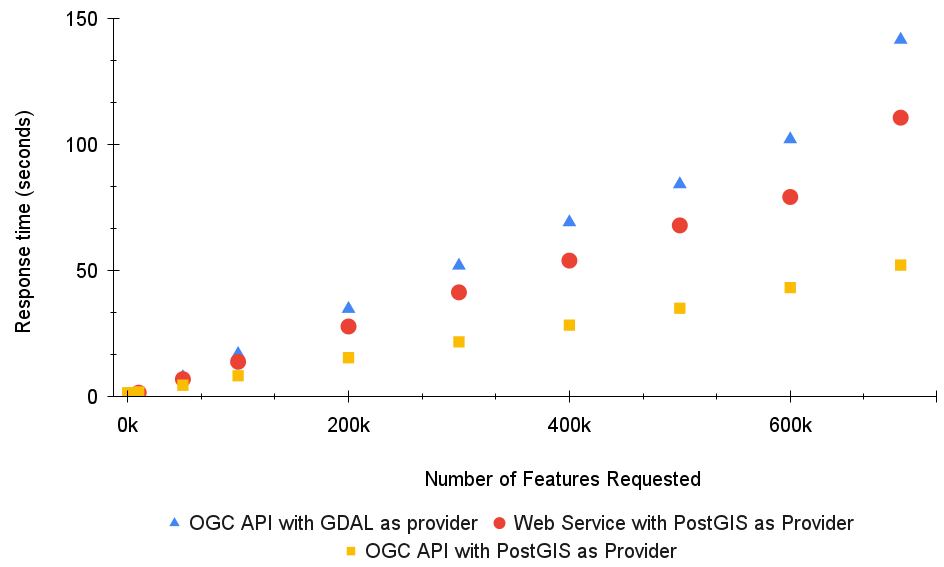
\includegraphics[width=0.8\textwidth]{img/dispersaoedificacao.png}
\caption{Average response time per maxFeatures requested for Edificacao}
\label{fig:timeperfeature_dispersaoedificacao}
\end{figure}

One-factor design can be used to compare a single factor with multiple alternatives and be able to compute the effect of each alternative. The table \ref{tab:onefactor} shows the three average response times for requests for 100,000 spatial data features obtained from three executions of the experiment for each approach. Computing the one-factor design we found that an average service requires 12955ms to respond to the chosen 100 thousand features of the dataset, corresponding to a 71M file. The API with GDAL as provider requires 7225.28ms more than the average service, a Web service requires 648.88ms more than the average service and the API querying the database requires 4874.77ms less than the average service. From the Analysis of Variance (ANOVA) we verified with 95\% confidence that the approach factor variation is significant.

\begin{table}[H]
\centering
\caption{Average Request Response for Three Executions }
\label{tab:onefactor}
\begin{tabular}{cc|c|c}
\cline{2-4}
\multicolumn{1}{l|}{}                                     & y                   & Mean     & \multicolumn{1}{c|}{Effect}  \\ \hline
\multicolumn{1}{|c|}{OGC API with GDAL as provider}       & (17424,16912,17209) & 17181,67 & \multicolumn{1}{c|}{4225,88} \\ \hline
\multicolumn{1}{|c|}{WFS with PostGIS as Provider} & (13793,13327,13694) & 13604,67 & \multicolumn{1}{c|}{648,88} \\ \hline
\multicolumn{1}{|c|}{OGC API with PostGIS as Provider} & (7962,8041,8240)    & 8081,00  & \multicolumn{1}{c|}{-4874,77}  \\ \hline
\multicolumn{1}{l}{}                                      & Total mean          & 12955,77 & \multicolumn{1}{l}{}         \\ \cline{3-3}
\end{tabular}
\end{table}

 From the linear regression model of the three alternatives discussed, which fits more than 98\% of the sample, %% ?? which achieved a correlation coefficient of 0.98 ? o coeficiente de determinação (R²) é de 98% no minimo pros tres, o quao bem o modelo prediz o tempo de resposta
 we observe the points of intersection where one approach becomes superior to the other. In Figure \ref{fig:comparetodos}, we can see that, from a dataset with 740,765 features, the API querying a Shapefile is superior to all other approaches up to 18,069 features, which corresponds to a 13MB file and 2.4\% of the requested dataset. Although initially the API querying the data in the database presents a significantly lower response time than the other approaches, the slope of its linear regression model is much smaller than that of the other approaches, so we can observe from the graph of the figure \ref{fig:comparetodos} that from 22,831 features requested onward, the response time of an API that directly queries the database is lower and grows more slowly than the other approaches.

\begin{figure}[H]
\centering
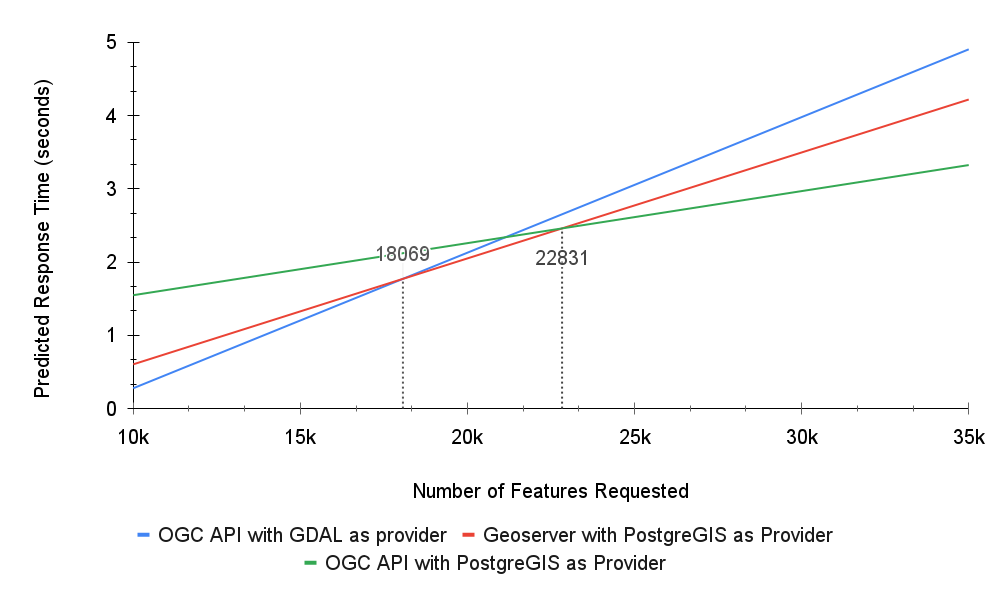
\includegraphics[width=0.9\textwidth]{img/comparetodos.png}
\caption{Linear regression for response time intersection}
\label{fig:comparetodos}
\end{figure}

\section{Data Type and Size Experiments}

To evaluate the impact of the variability in the size of the features and the type of spatial data geometry, we performed experiments to compare response times for varied workloads. 
%were performed that compare the file size and its response time for each fraction of each dataset. 
These experiments were performed using data storage in PostGIS for the API, using both large datasets. Figure \ref{fig:filesize} shows the file size increments for each requested fraction of the feature set for the two datasets, and Figure \ref{fig:timesize} shows the response time increase for the same fractions of the feature set.

For both approaches, a correlation coefficient above 99\% was calculated between the response time and the response size, indicating that as the response size increases, the response time increases linearly. Since both variables are related to the workload size, this result suggests that the workload size directly influences both the time and the response size.

\begin{figure}[H]
\centering
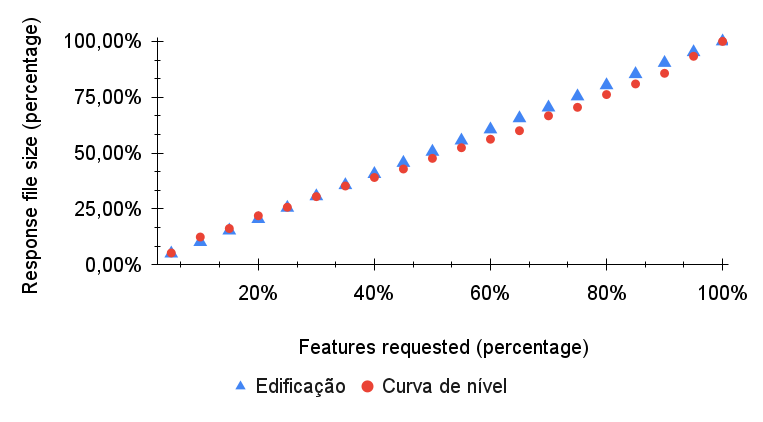
\includegraphics[width=0.7\textwidth]{img/comparesize.png}
\caption{Response file size per percentage of features requested for each dataset}
\label{fig:filesize}
\end{figure}

\begin{figure}[H]
\centering
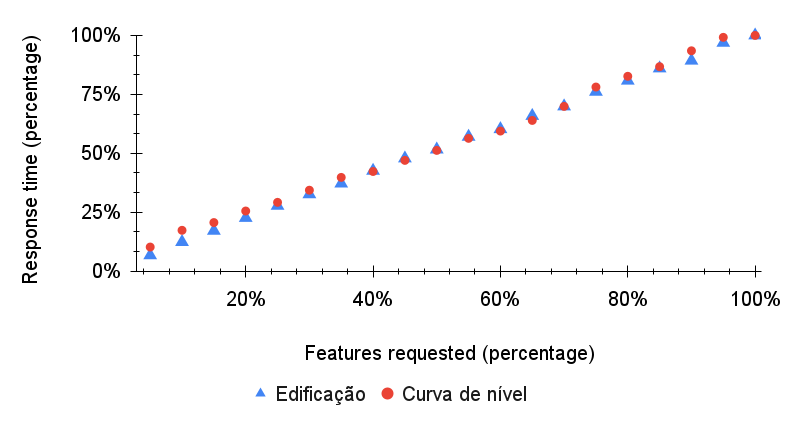
\includegraphics[width=0.7\textwidth]{img/comparetimeresponsecurvaedificacao.png}
\caption{Response time per percentage requested for each dataset}
\label{fig:timesize}
\end{figure}
